\documentclass[a4paper, 11pt, oneside]{report} 
\usepackage[utf8]{inputenc}
\usepackage[dutch]{babel}
\usepackage{diagbox}
\usepackage{amsmath}
\usepackage{amsfonts}
\usepackage{amssymb}
\usepackage{graphicx}
\usepackage{caption}
\usepackage[table,xcdraw]{xcolor}
\usepackage[toc,page]{appendix}
\usepackage{hyperref}
\usepackage{titlesec}
\usepackage{listings}
\usepackage{float}
\usepackage{tikz}
\usetikzlibrary{trees}
\usepackage{tikz-qtree}
\usepackage{graphicx}
\usepackage{fancyref}
\usepackage{wrapfig}
\usepackage{url}
\usepackage{pdflscape}
\usepackage{fancyvrb}
\usepackage{fancyhdr}
\graphicspath{ {Afbeeldingen/} }
\usepackage{subfig}
\usepackage{tabularx}
\usepackage{apacite}
\usepackage{longtable}
\usepackage{titlecaps}
%\usepackage[T1]{fontenc}
\usepackage{titlesec, blindtext, color}
\definecolor{gray75}{gray}{0.75}
\newcommand{\hsp}{\hspace{20pt}}
\usepackage{pdfpages}
\usepackage{booktabs}
\usepackage{listings}

\newcolumntype{L}[1]{>{\raggedright\arraybackslash}p{#1}}

\titleformat{\chapter}[hang]{\huge\bfseries}{\thechapter\hsp\textcolor{gray75}{|}\hsp}{0pt}{\Large\bfseries}

\makeatletter
\newcommand\tagreq[2]{#1\def\@currentlabel{#1}\label{#2}}
\makeatother

\def\checkmark{\tikz\fill[scale=0.4](0,.35) -- (.25,0) -- (1,.7) -- (.25,.15) -- cycle;} 
\def\figureautorefname{Figuur}
\def\subsectionautorefname{Subparagraaf}
\def\sectionautorefname{Paragraaf}
\def\chapterautorefname{Hoofdstuk}
\def\tableautorefname{Tabel}
\DeclareRobustCommand{\VAN}[3]{#2} % set up for citation

%% Sets page size and margins 
\usepackage[a4paper,top=3cm,bottom=3cm,left=3cm,right=3cm,marginparwidth=1.75cm]{geometry}

\definecolor{dkgreen}{rgb}{0,0.6,0}
\definecolor{gray}{rgb}{0.5,0.5,0.5}
\definecolor{mauve}{rgb}{0.58,0,0.82}

\lstset{frame=tb,
	language=Java,
	aboveskip=3mm,
	belowskip=3mm,
	showstringspaces=false,
	columns=flexible,
	basicstyle={\small\ttfamily},
	numbers=none,
	numberstyle=\tiny\color{gray},
	keywordstyle=\color{blue},
	commentstyle=\color{dkgreen},
	stringstyle=\color{mauve},
	breaklines=true,
	breakatwhitespace=true,
	tabsize=3
}

\author{M.W.J. Berentsen}
\font\myfont=cmr12 at 40pt
\title{\myfont Drone meshnetwerk simulatie}
\usepackage{titling}

\newcommand{\subtitle}[8]{%
	\posttitle{%
		\par\end{center}
	\begin{center}\large#1\end{center}
	\vskip0.5em
	\begin{center}\large#2\end{center}
	\begin{center}\large#3\end{center}
	\begin{center}\large#4\end{center}
    \begin{center}\large#5\end{center}
    \begin{center}\large#6\end{center}
    \begin{center}\large#7\end{center}
    \begin{center}\large#8\end{center}
	\vskip0.5em}%
}

\subtitle{Afstudeerverslag}{HAN Arnhem}{561399}{MWJ.Berentsen@student.han.nl}{Versie 1}{Alten Nederland B.V.}{Docent: J. Visch, MSc}{Assessor: ir. C.G.R. van Uffelen}

\setlength{\parindent}{0pt}
\setlength{\parskip}{5pt plus 2pt minus 1pt}



\hypersetup{colorlinks=true, urlcolor=red,citecolor=black,linkcolor=blue}  % Colours hyperlinks in blue, but this can be distracting if there are many links.
\setcounter{tocdepth}{2}



\begin{document}
\begin{figure}
\begin{center}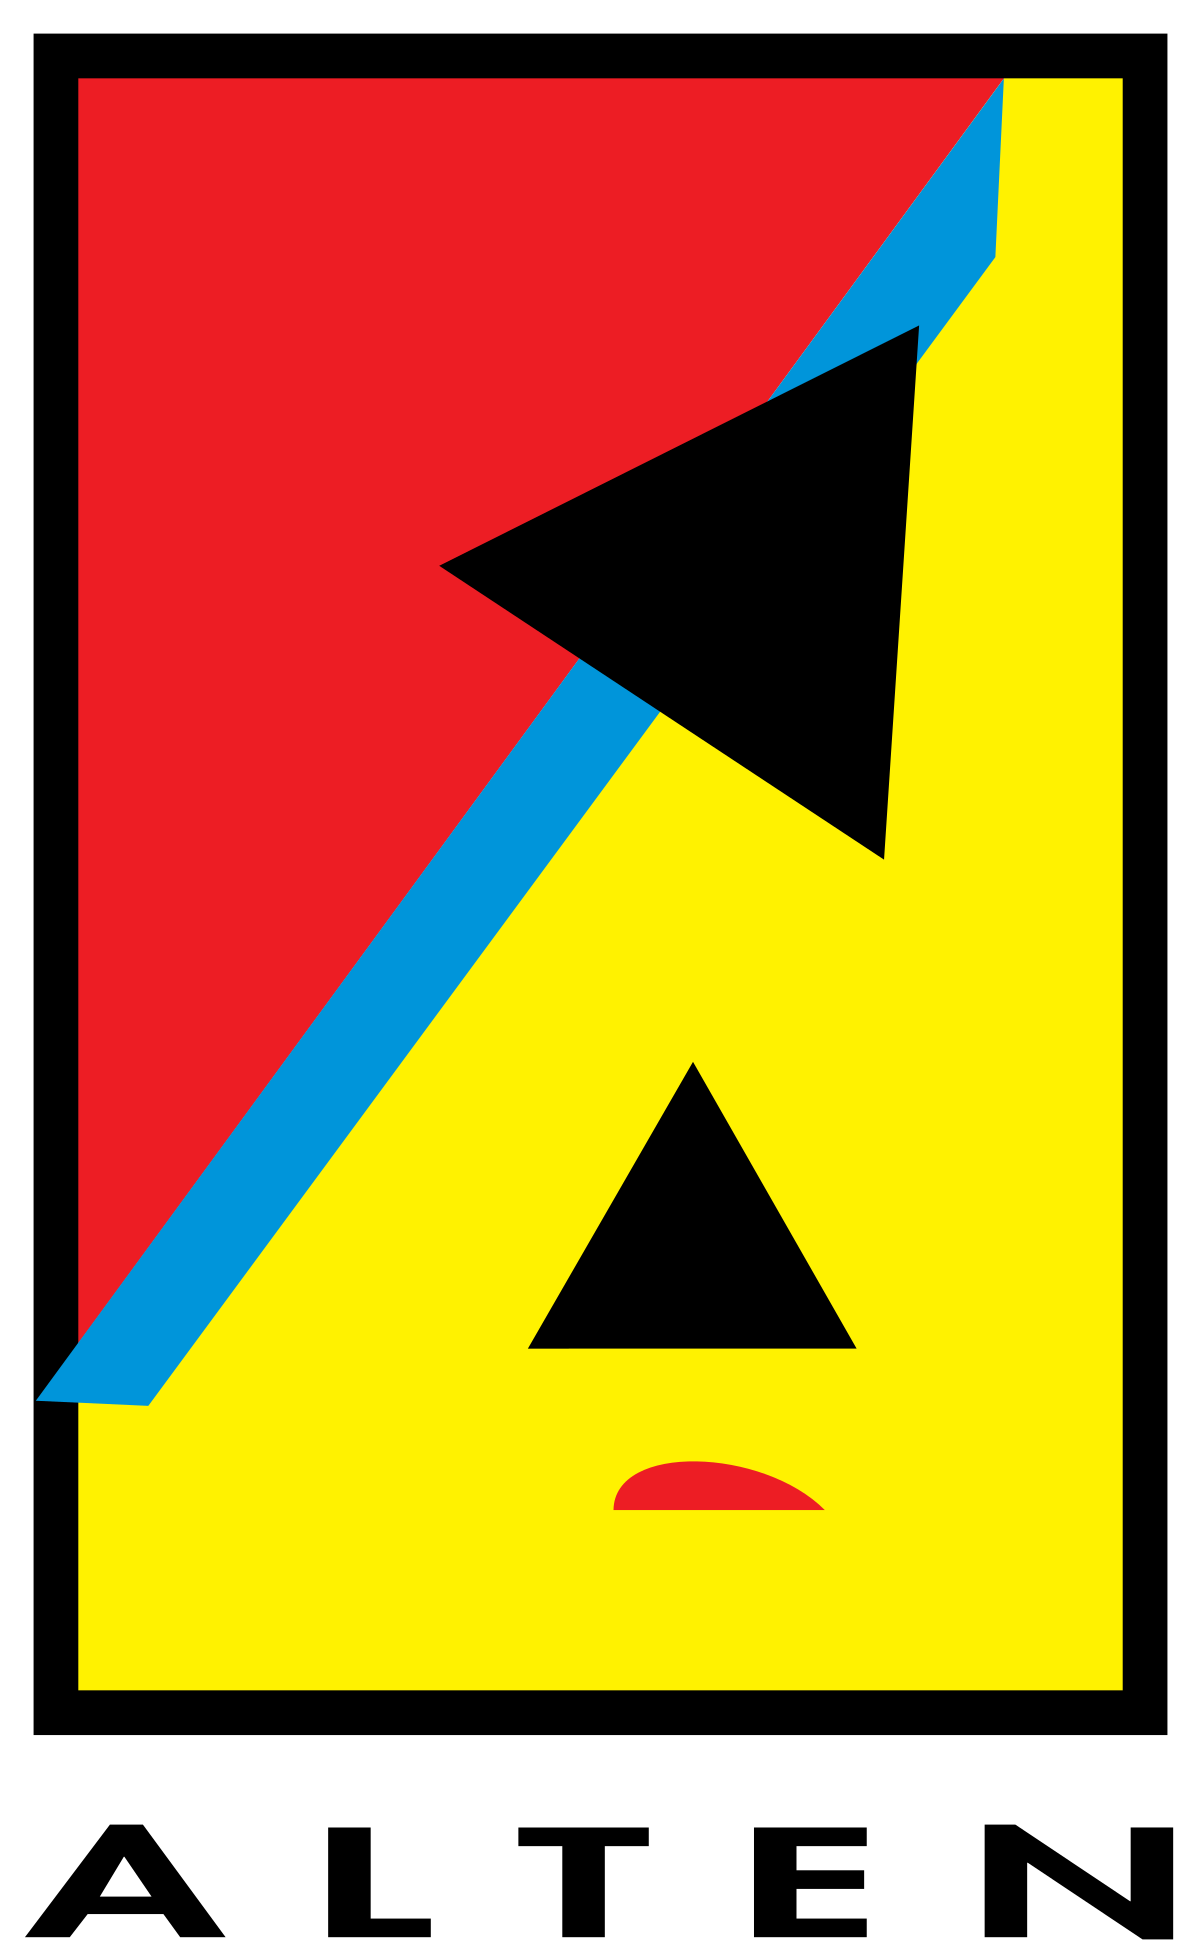
\includegraphics[scale=0.1]{alten}\end{center}
\end{figure}
\maketitle

%\section*{Voorwoord}
%\addcontentsline{toc}{section}{\protect\numberline{}Voorwoord}
%\pagebreak
\chapter*{Managementsamenvatting}\label{sec:managementsamenvatting}
Het doel van "Drone meshnetwerk simulatie"\ is het zetten van de eerste stap in de ontwikkeling van het
dronenetwerk. Hiervoor is de volgende opdracht opgesteld:
\begin{quotation}
	\textit{Maak een netwerkmodule voor een drone die het mogelijk maakt om meerdere drones onderling te voorzien van een zelf herstellend meshnetwerk. Maak deze module na in een simulatie die geschikt is om meer dan 100 drones te simuleren waarvan het netwerk zich gelijk gedraagt zodat er verdeelalgoritmes getest kunnen worden.}
\end{quotation}

Deze opdracht is uitgevoerd door eerst kwantitatief onderzoek uit te voeren.

Eerst is er gekeken welke simulatiesoftware gebruikt moet worden voor het simuleren van het dronenetwerk.
Er is gekozen om dit te doen in de softwarecombinatie ROS + Gazebo omdat dit het hoge aantal drones kan verwerken maar wel toegang heeft tot een physics engine.

Om een betere keuze te kunnen maken welke hardware gebruikt zou moeten worden voor onderlinge communicatie is er eerst gekeken wat de grootte van de payload is die verstuurd zou moeten worden om nuttig te zijn in een netwerk.

Vervolgens is gekeken naar welke hardware gebruik zou moeten worden voor de onderlinge communicatie. Hier is gekozen voor een Arduino UNO een microcontrollerbord met een daarop aangesloten radio module nRF24l01+.

Hierna is er een keuze gemaakt welke routeringstechniek gebruik moet worden waarop de conclusie was om een hybide routeringstechniek te gebruiken die als basis een reactieve protocol heeft met als toevoeging dat routes wel opgeslagen worden. De student heeft een aangepaste versie van de Lightweight Mobile Routing Protocol(LMR) toegepast. 

Er is een conclusie getrokken dat het voor dit project niet nodig is om een drone volledig correct te implementeren. Een abstracte versie zal voldoen. Hier zijn regels over opgesteld waar deze aan zou moeten voldoen. 

Om de opdracht uit te kunnen voeren heeft de student een simulatie gemaakt waar drones zich kunnen voortbewegen en zich conform de casus opgesteld in het plan van aanpak kunnen verdelen. De drones volgen het gedrag van een meshnetwerk en er is applicatie aanwezig om op realistische wijze verzoeken te sturen naar de drones voor verplaatsing. 

De opgeleverde software wordt onderbouwt in het software design document en de software requirements specificatie.

\tableofcontents
\clearpage
%\section*{Begrippenlijst}

% Please add the following required packages to your document preamble:
% \usepackage[table,xcdraw]{xcolor}
% If you use beamer only pass "xcolor=table" option, i.e. \documentclass[xcolor=table]{beamer}
%\begin{table}[H]
%\centering

%\label{begrippen}
%\begin{tabular}{|l|l|}
%\hline
%\rowcolor[HTML]{C0C0C0}
%Term        & Omschrijving                                                         \\ \hline
%term        & Omschrijving                                                      	\\ \hline

%\end{tabular}
%\caption{Begrippenlijst}
%\end{table}

%\clearpage

%\section*{Samenvatting}
%\addcontentsline{toc}{section}{\protect\numberline{}Samenvatting}
%\pagebreak



\chapter{Inleiding}\label{sec:inleiding}

Dit document is het eindverslag van de afstudeeropdracht genaamd "Drone meshnetwerk simulatie".
De simulatie simuleert een netwerk van drones die onderling met elkaar verbonden zijn door het gebruik van meshnetwerk technieken.
De simulatie dient een tweevoudig doel: Allereerst kunnen er met de simulatie verdeelalgoritmes getest worden. Het tweede doel is het optimaliseren het netwerk om zo de stabiliteit hiervan te kunnen optimaliseren.

Het doel van dit document is het aantonen van de volwassenheid van het project en de opgeleverde deelproducten conform de vijf beroepscompetenties.
Dit wordt bewezen aan de hand van de producten die zijn gerealiseerd of handelingen die zijn verricht tijdens de afstudeerstage. In dit document wordt regelmatig verwezen naar andere documenten zoals het plan van aanpak, onderzoekrapport, software design document en de software requirements. Dit wordt gedaan omdat deze documenten ook aantonen dat de student zich HBO waardig heeft gedragen tijdens dit project.  

Het eindverslag is zo opgebouwd dat dit de opdracht, context en eindproducten beschrijven en hoe de student bezig is geweest conform de vijf beroepscompetenties.

\begin{itemize}
	\item Bedrijfsbeschrijving.
	
	Hier wordt het bedrijf omschreven waar de opdracht wordt uitgevoerd en het team wordt besproken.
	\item Opdrachtomschrijving.
	
	Dit hoofdstuk wordt gebruikt om de aanleiding, probleemstelling, doel, opdracht en resultaten toe te lichten.
	
	\item Methoden, technieken, platforms, tools.
	
	De gebruikte methoden, technieken, platforms en tools worden in dit hoofdstuk toegelicht. Hier gaat het met name om waarom er een keuze is gemaakt en wat de alternatieven waren. De projectmanagement methodiek blijft hierbuiten aangezien deze al wordt toegelicht in het plan van aanpak.
	
	\item Uitvoer projectplan.
	
	Hier wordt het plan van het project gereflecteerd. Er wordt gekeken wat er volgens planning ging maar wat ook niet en waarom dat dan zo was.
	
	\item Proces en aanpak
	
	In het hoofdstuk proces en aanpak wordt er gekeken welke stappen zijn genomen en wat hun verband is met betrekking tot het proces
	
	\item Resultaten
	
	Wat is er opgeleverd en voldoet het aan de opgestelde kwaliteitseisen gesteld in het plan van aanpak. Als er afwijkingen zijn worden die ook in dit hoofdstuk besproken.
	
	\item Evaluatie 
	
	Dit hoofdstuk geen inzicht met betrekking tot het proces, producten en resultaten en het functioneren van de student.
	
	\item Conclusie
	
	Het afsluitende hoofdstuk behandeld wat de student heeft opgeleverd en of dit voldoet aan de doelstelling van het project.
	Als er afwijkingen zijn wordt dit ook beschreven.
	Tenslotte worden er een advies gegeven aan het bedrijf in welke vervolgstappen zij zou kunnen nemen.
	
\end{itemize}

\chapter{Bedrijfsbeschrijving}\label{sec:bedrijfsbeschrijving}

Alten is een multinational met +- 25.000 medewerkers wereldwijd en is van origine begonnen in 1988 en in de eerste tien jaar organisch gegroeid totdat ze in 1999 een beursgenoteerd bedrijf werden.
Vanaf het jaar 2000 hebben ze de eerste internationale dochterondernemingen gestart waarvan de eerste in Nederland in 2002 was (dit was een overname van een ander bedrijf).
In 2005 is Alten NL tot leven geroepen die zich focust op het geven van technische consultancy.
Op dit moment heeft Alten NL ongeveer 650 medewerkers, waarvan elk persoon minimaal een bachelors diploma heeft, 30-40\% een masters diploma, en 10-15\% een PhD heeft.
Dit maakt Alten dan ook een vooruitstrevend bedrijf die zich altijd bezig houdt met innoverende technologieën en probeert vooraan te staan
wanneer een nieuwe technologie doorbreekt.

Anno 2019 heeft Alten vier filialen in Nederland: Amstelveen, Capelle a/d IJssel, Eindhoven en Apeldoorn.
De student is geplaatst bij het filiaal in Apeldoorn.

Zoals gezegd focust Alten zich vooral op technologie en dat is niet enkel beperkt tot software want zo hebben ze namelijk ook: Technische Software, mechatronica, IT test services, Business Intelligence \& Analytics en Digital Enterprise.
Alten faciliteert voornamelijk in consultancy (85\% van alle werkzaamheden) maar doen ook ‘in huis’ projecten voor haar klanten.

Het bedrijf heeft zes kernwaarden die als volgt luiden: kennis netwerkers, technologie, streef hoog, open en betrokken, mensen en plezier/lol.
Alten benadrukt dat het belangrijk is om je kennis te delen met anderen (want samen sta je sterker), dit proberen zij
te bereiken met de zogeheten kennisgroepen. 

\section{Het team}\label{sec:het-team}
Het team betrokken bij dit project wordt hier kort omschreven.

\paragraph{Uitvoerend student: Maurice Berentsen}

Het afstudeerproject is uitgevoerd door de student Maurice Berentsen. 
Hij is een student aan de Hogeschool van Arnhem en Nijmegen. 
Zijn belang bij dit project is tweezijdig. 
Enerzijds voert Maurice dit project uit om aan te tonen hij de vijf beroepscompetenties beheerst en daarom waardig is voor het ontvangen van het Bachelor diploma Technische Informatica. 
Anderzijds voert hij dit project uit omdat hij een interesse heeft naar mobiele meshnetwerken en dit na het behalen van zijn diploma in de praktijk zou willen brengen bij een toekomstig opdrachtgever. 

\paragraph{Technisch manager: Hugo Logmans}

Hugo Logmans is de technische manager voor Alten oost. Hij begeleidt de consulenten in hun carrière en werk. Sinds 1999 is Hugo werkzaam als ontwikkelaar en heeft hier dus bijna 20 jaar ervaring in. Zijn belang in dit project is het onderzoeken wat er toegevoegd kan worden in een meshnetwerk om het ondervinden van uitgevallen punten snel te achterhalen.

\paragraph{Business manager: Jeroen Nijenhuis}
Jeroen Nijenhuis is business manager van de locatie oost. Hij zorgt voor contactafhandeling naar bijvoorbeeld p\&o. Bij hem kan de student terecht voor vragen buiten het vakgebied. Zijn belang bij het project is het zorgen dat de overgang van de schoolomgeving naar een bedrijfsomgeving goed verloopt 

\paragraph{Bedrijfsbegeleider: Hugo Heutinck}

Hugo Heutinck is een werknemer van Alten. Hij heeft in 2003 een master behaald in Computer Technics en is sindsdien aan het werk als (embedded) software engineer. Hij is een specialist in Linux en heeft voert de rol uit van SCRUM master. Zijn belang bij dit project is het begeleiden van de student.

\paragraph{Begeleidende leraar: Jorg Visch}
 
Jorg Visch is een leraar op de Hogeschool van Arnhem en Nijmegen werkzaam binnen het lerarenteam van de uitstroomrichting Embedded Software Developer. Hij is leraar van Maurice geweest tijdens het semester Internet of Things. Zijn belang bij dit project is begeleiden van Maurice tijdens het afstuderen.

\paragraph{Assessor: Chris van Uffelen}

Chris van Uffelen is een collega van Jorg Visch en werkzaam in hetzelfde team. Hij heeft Maurice begeleidt tijdens het Object-oriented Software and Modelling project. Zijn belang bij dit project is het beoordelen of het project waardig is aan het verschaffen van het Bachelor diploma Technische Informatica. Hij doet dit in samenwerking met Jorg Visch. 


\chapter{Opdrachtomschrijving}\label{sec:opdrachtomschrijving}
Het doel van Alten is om onderling verbonden drones te kunnen verdelen om zo een netwerk op te kunnen bouwen over een gebied. 
Alten wil dat dit netwerk zichzelf kan onderhouden door te reageren op uitval of een slechte verbinding door de één of meerdere drones te herverdelen.

\section{Probleem}\label{sec:probleem}
Op dit moment is Alten in het bezit van drones maar deze kunnen niet met elkaar communiceren.
Om te kunnen communiceren moet er een netwerkmodule toegevoegd worden aan elke drone.
Alten wil grote netwerken kunnen opbouwen die robuust zijn en daarom wil zij gebruik maken van een zelf herstellend meshnetwerk.
Hoewel er al meerdere oplossingen bestaan in het gebruik van meshnetwerken wil Alten het zelf herstellend vermogen vergroten. 
Daarom wil Alten dat de focus van de netwerkmodule ligt op het snel detecteren van uitval van punten in het netwerk zodat daar adequaat op gereageerd kan worden.
Adequaat reageren kan op twee manieren volgens Alten.
De netwerkmodule kan een ander netwerkpunt zoeken om via dat punt te communiceren, als deze niet beschikbaar is het alternatief om de drones opnieuw te verdelen.
Het autonoom fysiek kunnen verplaatsten van de netwerkpunten is dan ook de uitbreiding die Alten wil toevoegen aan het zelf herstellend vermogen.
Alleen wat is een efficiënte manier van herverdelen?
Het makkelijkste is om alle drones terug naar hun start punt laten vliegen maar dit zou betekenen dat het netwerk op dat moment niet beschikbaar is en het zou ook nog eens onnodig veel stroom verbruiken.

Om algoritmes te testen voor het verdelen van de drones is een simulatie de oplossing.
Hierbij is het dus ook van belang dat een simulatieomgeving zich realistisch gedraagt. 
Om realistisch gedrag na te bootsen moeten de virtuele netwerk modules zich in de simulatie zich net zo gedragen als in het echt.

\section{Doelstelling}\label{sec:doelstelling}
Het doel van dit project is het zetten van de eerste stap in de ontwikkeling van het dronenetwerk.
De eerste stap is ontwikkelen van een netwerkmodule voor het onderling verbinden van drones.
Het is van belang dat het meshnetwerk van de drones snel kan reageren op uitval van netwerkpunten.
Deze netwerkmodule moet zowel virtueel als fysiek gerealiseerd worden in dit project.

Voor het virtueel realiseren van de netwerkmodule moet een simulatie gebruikt worden. 
Omdat er nog geen simulatiesoftware beschikbaar is wil Alten dat de student uitzoekt welke simulatiesoftware geschikt is voor het simuleren van meer dan 100 drones.
Vervolgens kan de student deze software gebruiken om de virtuele netwerkmodules te testen.

\section{Opdracht}\label{sec:opdracht}
De opdracht van dit project is de ontwikkeling van meerdere producten die bijdragen aan het behalen van het doel. 

De student moet een prototype maken van een netwerkmodule die het onderlinge meshnetwerk verzorgt en zichzelf kan herstellen bij uitval of slecht signaal.
Wanneer er geen alternatieve communicatie route mogelijk is moet de module de drone een instructie uitsturen om zich te herpositioneren.

De student moet een simulatie opzetten waarin de netwerkmodules verplaatst kunnen worden in een vrije ruimte. 
In de simulatie moet het mogelijk zijn om de netwerkmodules te verplaatsen aan de hand van hun $X$, $Y$ en $Z$ as zodat er verdeelalgoritmes getest kunnen worden.  
De netwerkmodules moeten in de simulatie kunnen uitvallen en de onderlinge afstand heeft effect op de virtuele signaalsterkte.
De simulatie moet aan de hand van een script herhaalbaar zijn met eenzelfde resultaat.

Alten wil graag dat de simulatiesoftware gebruik maakt van Robot Operating System (ROS) als middleware. 
Dit wil Alten omdat zij al kennis heeft in ROS maar nog niet in combinatie met drones en mesh netwerken en door het begeleiden hier ervaring in opdoet.
Het ervaring opdoen in ROS is geen doel van dit project en de student hoeft zich hier niet op te concentreren.

Hoewel de keuze van de simulatiesoftware zich concentreert op het simuleren van een dronenetwerk zal de student alleen de netwerkmodule toevoegen aan de simulatie. 
De student zal zich dus niet specialiseren in het realistisch simuleren van drones.

Het project is geslaagd als een prototype van het meshnetwerk is opgeleverd samen met een simulatie waarin het mesh netwerk getest kan worden met verschillende verdelingsalgoritmes.

\subsection{Casus}\label{sec:casus}
Om het doel waar naartoe gewerkt moet worden te voorzien van een richting heeft Alten een casus bedacht.
Deze casus wordt hieronder toegelicht in een schets en is voorzien van individuele situaties.
Er wordt gedrag omschreven voor een simpel algoritme van het herstel van het meshnetwerk om aan te tonen dat dit getest kan worden in de simulatie.
In de casus blijft het vlieggedrag buiten de scope.


In de schets van \autoref{fig:schetsNetwerk} wordt er vanuit gegaan dat elke drone een directe vluchtroute heeft met zijn verbonden netwerkpunt.
De verbindingen zijn gemaakt  om de casus uit te leggen en volgen dus niet de realistische verbindingen die ze zouden hebben op basis van locatie.
\begin{figure}[H]
	\begin{center}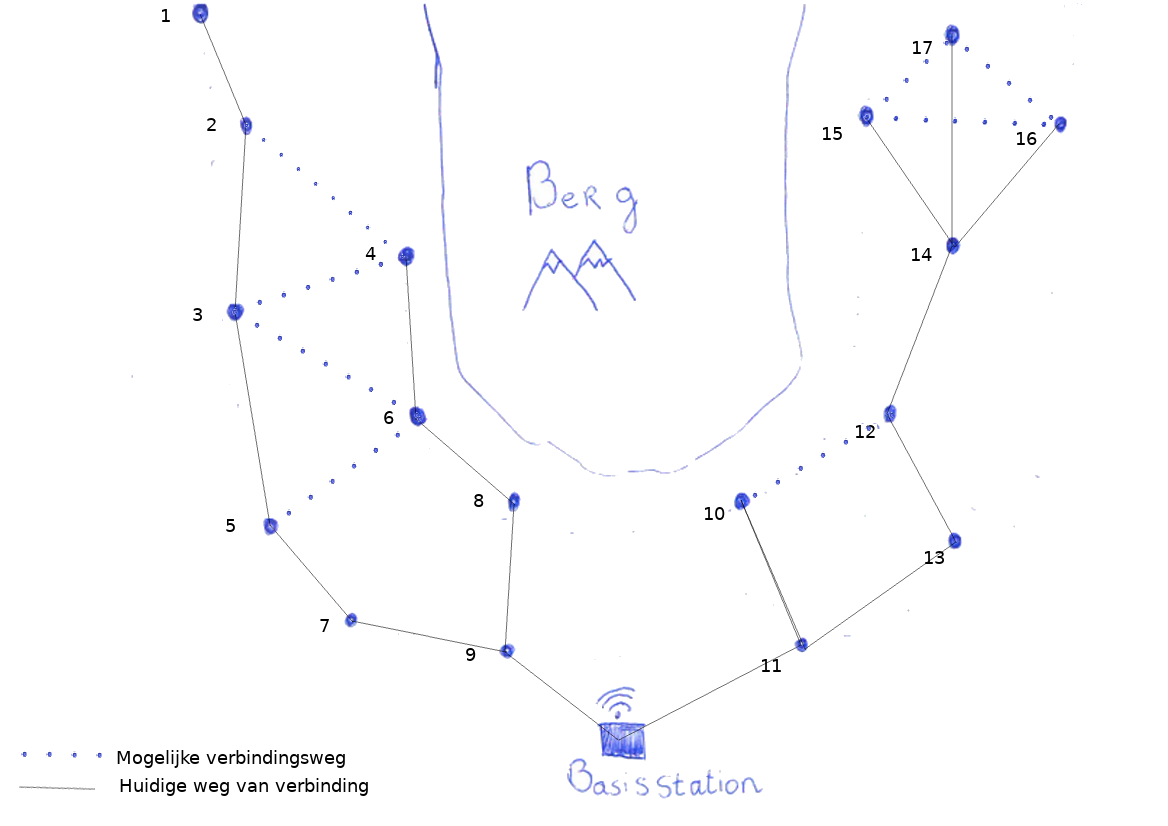
\includegraphics[width=0.61\linewidth]{schetsNetwerk}\end{center}
	\caption{Schets van casus netwerk}
	\label{fig:schetsNetwerk}
\end{figure}
In de casus komen de volgende situaties apart voor:

\begin{itemize}
	\item Punt 2 valt uit waardoor punt 1 geen verbinding meer heeft met het basisstation. Het verwachte resultaat is dat drone 1 zich verplaatst naar de positie van drone 2 en zo het netwerk herstelt.
	\item De bovenstaande situatie gebeurd. Tijdens het verplaatsen van punt 1 herstelt punt 2 zich weer. Het verwachte resultaat is dat punt 1 weer terug  keert naar zijn oude positie.
	\item Punt 3 valt uit waardoor punt 1 en 2 geen verbinding meer hebben met het basisstation. Het verwachte resultaat is dat drone 2 een nieuwe verbinding aangaat met drone 4.
	\item Punt 14 valt uit waardoor punt 15, 16 en 17 geen verbinding meer hebben met het basisstation. Het verwachte resultaat is dat de drones 15, 16 en 17 eerst met elkaar verbinden, vervolgens zal één van de drones zich verplaatsen naar punt 14. 
\end{itemize}

\section{Op te leveren resultaten voor het bedrijf en school}\label{sec:op-te-leveren-resultaten-voor-het-bedrijf-en-school}

Aan het einde van het project levert de student de volgende producten op aan het bedrijf:

\begin{itemize}
	\item Simulatiesoftware met netwerksimulatie
	\item Prototype meshnetwerk module.
	\item Broncode van de bovenstaande producten. 
	\item SRS (Software Requirement Specification)
	\item SDD (Software Design Document)
	\item Onderzoeksverslag
\end{itemize}

Aan het einde van het project levert de student het bovenstaande plus een projectverslag op aan de Hogeschool van Arnhem en Nijmegen.


\chapter{Methoden, technieken, platforms, tools}\label{sec:methoden-technieken-platforms-tools}
Wat gebruik je en waarom, overwogen alternatieven, waarom is de keuze gevallen op die
tool/techniek/platform. En dan niet zozeer (of alleen) de project(management)methodiek, die is al
uitgebreid verantwoord in het PvA als het goed is.

\chapter{Uitvoer projectplan}\label{sec:uitvoer-projectplan}
Wat was het plan, hoe heb je dat uitgevoerd. Waar zitten de afwijkingen en waarom? Beperkt tot
inhoudelijk relevante zaken.
Dit hoofdstuk behandeld hoe het plan van het project is uitgevoerd, het zal eerst kort toelichten wat het plan was. Vervolgens zal er reflectie op het plan plaats vinden.

\section{Het plan}\label{sec:het-plan}

\section{Reflectie}\label{sec:reflectie}


\chapter{Proces en aanpak}\label{sec:proces-en-aanpak}
Wat heb je gedaan en waarom? Wat is het verband tussen de verschillende stappen die je genomen hebt in
het proces?
\chapter{Resultaten}\label{sec:resultaten}

%Inhoudelijk, wat heb je opgeleverd, met welke kwaliteit? Was dit ook volgens plan? Ben je afgeweken en zo
%ja waarom?
%(Deze laatste drie kunnen ook geïntegreerd worden)
In de dit hoofdstuk worden de opgeleverde producten behandeld en beoordeeld op hun kwaliteit.

\section{Plan van aanpak}\label{sec:plan-van-aanpak}
Het eerste product die ik heb opgeleverd was het plan van aanpak.
Het product kreeg zijn echte waarde na de feedback op het conceptplan.

Het eerste plan was nog niet concreet genoeg in wat opgeleverd zou ging worden. 
Dit was dan ook in grote lijnen wat de feedback was vanuit de begeleiders van school.

Na het verwerken van de feedback was het plan veel gerichter in wat opgeleverd zou moeten worden.
Het plan wat er nu ligt zou uitgevoerd kunnen worden door elke ICT'er met de juiste vaardigheden.
De kwaliteitseis die ik gesteld heb aan het plan van aanpak was dat het moest omschrijven wat het plan van de student is en dat het voldoet aan het feedbackformulier projectplan van het \citeauthor{HANfeed} \citeyear{HANfeed}. Deze kwaliteitseisen zijn voldaan wat dus betekend dat het op papier voldoet aan alle kwaliteit.

Wat in mijn ogen nog beter bewijst dat het plan van aanpak een document van kwaliteit is, is dat ik gedurende het project regelmatig het plan erbij heb gepakt om beslissingen op te baseren en kwaliteit van andere producten mee te meten.

\section{Broncode}\label{sec:broncode}
De code geschreven voor dit project heeft veel aandacht van mij gekregen. 
Er heeft veel moeite gezeten in het gebruik van Doxygen om dit volledig compleet te houden.
Als resultaat geeft dan wel een complete documentatie bij het generen van de documentatie. 

Wat wel is uitgevoerd maar naar mijn mening te weinig is toegepast is het gebruiken van unittesten.
Dit is weinig gebruikt omdat veel code een communicatie uitvoert naar een andere netwerkcomponent.
Er kunnen wel unittesten voor geschreven worden maar het opzetten van een basis voor zulke testen kost veel tijd.
Toch zou ik Alten wel adviseren als ze dit project voortzetten om hier in te investeren.
Het schrijven van een routeringstechniek is een complex proces die in de huidige implementatie nog problemen kan geven.
Het breder toepassen van unittesten zou de kwaliteit van het meshnetwerk zeker ten goede komen. 

De componenten die gebruikt worden zijn goed met elkaar aangesloten waarbij er een uitzondering is dat er een adapter gebruikt wordt om de gesimuleerde drone op een Arduino aan te sluiten. 

Wat ik jammer vind maar niet mogelijk was in het project was dat er geen buildserver beschikbaar was waar een geavanceerde codeanalyse tool aan gekoppeld zit zoals coverity of sonarqube. Wel is er in het project gebruik gemaakt van de statische codechecker CPPcheck. Hoewel het geen maatstaaf is hier nul meldingen op te krijgen in verband met false positives is dat in het geval van dit project wel zo. 

  
\section{Onderzoeksrapport}\label{sec:onderzoeksrapport}

Het onderzoeksverslag is een verslag die naar mijn mening inhoudelijk niet voldoende gespreide aandacht heeft gekregen. Hoewel het misschien de onderzoeksvraag beantwoord is er duidelijk te merken dat het literatuur onderzoek naar de te gebruiken hardware en simulatiesoftware veel meer tijd heeft gekregen dan de rest van het document.

De hoofdvraag gesteld in het onderzoek is relevant omdat het helpt met het uitvoeren met de specifieke opdracht.
De deelvragen daarentegen zijn niet allemaal even sterk uitgewerkt. 
Zo is er de vraag wat nodig is om een abstracte drone te representeren. 
Hier had ik veel onderzoek naar kunnen doen maar dit heeft geen meerwaarde. 
Een kort overleg voldoet in dit onderwerp ook waarin besproken is van wat moet de gesimuleerde drone allemaal kunnen.

Op zich is dit gezien de beschikbare tijd een prima keuze maar het haalt de kwaliteit van het onderzoek wel naar beneden.

Wat goed is gedaan in het onderzoek is het gebruik van bronnen, zo zijn ze voornamelijk gebaseerd op wetenschappelijke artikelen en zijn ze ruim aanwezig.

Verder merkte ik dat het fijn is voor het bedrijf dat ik de onderzoeksmethode geleerd op de HAN nog toegelicht heb aangezien lang niet iedereen hiermee bekent is. Ook het toelichten hoe onderzoek op de HAN werkt is goed onderbouwt toegelicht.
  


\section{Simulatiesoftware}\label{sec:simulatiesoftware}
Tegen het einde van het project werd de simulatiesoftware opgeleverd. 
Dit was het product waar de meeste focus en ontwikkeling in heeft gezeten.
Dit was initieel niet het plan omdat er meer focus op het hardware prototype zou liggen.
Gedurende het project werd de urgentie van de simulatie software steeds duidelijker.

Door het gebrek aan voldoende hardware kon er niet goed getest worden hoe het netwerk zich zou gedragen bij een hoog aantal nodes.
Daarom is er gekozen om de simulatie een hogere prioriteit te geven zodra de gesimuleerde communicatie realistisch genoeg was.

Een tegenvaller van de simulatie in Gazebo was dat voor het simuleren van 100 drones en dit visueel te maken een computer met een dedicated GPU nodig is. Dit was vooraf niet verwacht omdat de drones in de simulatie alleen maar vliegende blokjes zijn. 

Het opgeleverde product voldoet wel aan de wens van Alten zij wil namelijk verdeelalgoritmes kunnen testen waarbij de drones op een realistische wijze worden aangestuurd en dat is ook opgeleverd.  Verder is de simulatie voorzien van voldoende documentatie.  

\section{Hardwareprototype}\label{sec:hardwareprototype}


\section{Software design document}\label{sec:software-design-document}
\section{Software requirements specificatie}\label{sec:software-requirements-specificatie}

\chapter{Evaluatie}\label{sec:evaluatie}

Evaluatie/ Reflectie / Situaties (STARR)
Inzichten!
Inzichten mbt proces, producten en resultaten, èn het eigen functioneren. middels een methode als STARR.
Die methode moet dan wel goed toegepast worden.

\chapter{Conclusie}\label{sec:conclusie}
Inhoudelijk, wat heeft het project opgeleverd, zet dat af tegen de doelstelling, heb je die gehaald?
Afwijkingen beschrijven. Welke vervolgstappen kan het bedrijf nog nemen?

\section{Advies vervolg project}\label{sec:advies-vervolg-project}


\bibliographystyle{apacite}
\bibliography{bilbliography.bib}

\clearpage
\appendix
%\chapter{Schets voor casus drone netwerk}

\end{document}